\section{Background and Motivation}
\label{sec:background}

\begin{figure}[t]
   \centering
   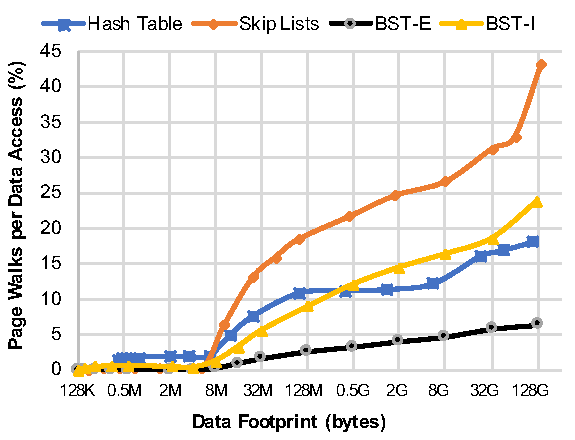
\includegraphics[width=1.0\columnwidth]{graphs/pagewalks.pdf}
   \caption{Frequency of page walks as a function of memory size.}
   \label{fig:pagewalks}
\end{figure}


\begin{table*}[]
\centering
\caption{Comparison of SpryVM with previous approaches for reducing
  virtual memory overhead. For protection/security, we show
  tick/cross-marks for each of those cases. Coarse-grained protection
  is indicated with a cross, as is lower entropy in virtual address
  bits.}
\label{table:vms}
\begin{tabular}{
>{\columncolor[HTML]{FFFFFF}}l |
>{\columncolor[HTML]{FFFFFF}}c |
>{\columncolor[HTML]{FFFFFF}}c |
>{\columncolor[HTML]{FFFFFF}}c |
>{\columncolor[HTML]{FFFFFF}}c |}
\cline{2-5}
\multicolumn{1}{c|}{\cellcolor[HTML]{FFFFFF}}                           & Programmability  & Performance and Efficiency & Flexibility & Protection/Security \\ \hline
\multicolumn{1}{|l|}{\cellcolor[HTML]{FFFFFF}Multi-page mappings~\cite{pham:colt, pham:increasing}}       & \cmark              & \xmark                          & \cmark           & \cmark \ \cmark     \\ \hline
\multicolumn{1}{|l|}{\cellcolor[HTML]{FFFFFF}Transparent Huge Pages~\cite{transparenthugepages}}    & \cmark               & \xmark                          & \cmark           & \xmark \ \cmark      \\ \hline
\multicolumn{1}{|l|}{\cellcolor[HTML]{FFFFFF}Libhugetlbfs~\cite{lighugetlbfs}}              & \xmark                & \xmark                          & \cmark           & \xmark \ \cmark      \\ \hline
\multicolumn{1}{|l|}{\cellcolor[HTML]{FFFFFF}Direct Segments~\cite{basu:efficient}}           & \xmark              & \cmark                          & \xmark           & \xmark \ \xmark      \\ \hline
\multicolumn{1}{|l|}{\cellcolor[HTML]{FFFFFF}Redundant Memory Mappings~\cite{karakostas:redundant}}  & \cmark             & \xmark                          & \xmark           & \xmark \ \xmark      \\ \hline
\multicolumn{1}{|l|}{\cellcolor[HTML]{FFFFFF}Direct-mapped Mappings~\cite{picorel:near-memory, haria:devirtualizing}}         & \cmark       & \cmark                          & \xmark           & \xmark \ \xmark     \\ \hline
\multicolumn{1}{|l|}{\cellcolor[HTML]{FFFFFF}SpryVM (Our Approach)}                    & \cmark                       & \cmark               & \cmark           & \cmark \ \cmark     \\ \hline
\end{tabular}
\end{table*}

\subsection{Goals for VM in Large Heterogeneous Systems}
When buiding VM support for accelerators, it is important to identify
design goals for the its operation. Like prior work
\cite{haria:devirtualizing}, we identify the following as key goals in
our design:

\begin{itemize}
        \item \textbf{Programmability.} The widespread adoption of
          accelerators rests on the usability and familiarity of their
          programming models. Unified virtual memory between CPUs and
          accelerators are one way of achieving this in a manner that
          simplifies data sharing, eliminating the need for
          hand-managed data copying and marshaling. Ideally, we wish
          to preserve all the benefits typically associated with VM
          like memory protection and isolation, and flexibility of
          sharing parts of the address space among processes.

        \item \textbf{Flexibility.} Traditional VM imposes no
          restrictions on virtual-to-physical page mapping
          relationships. This is valuable to support any level of
          system memory fragmentation, application multi-tenancy,
          memory allocation strategies transparent to programmers, as
          well as the integration of features such as paging and
          copy-on-write (CoW).

        \item \textbf{Safety and Security.} Direct access to physical
          memory is generally not acceptable nor desirable. Such
          memory management approaches cannot prevent malicious or
          erroneous memory accesses and prohibits sharing accelerators
          across different processes with proper
          isolation~\cite{haria:devirtualizing}. Furthermore, the
          entropy in address mapping must be as high as possible to
          reduce vulnerability to security attacks.

        \item \textbf{Performance and Efficiency.} Crucially, all the
          goals listed thus far must be achievable without excessive
          performance or area overheads in hardware. In other words,
          address translation must provide near-zero performance
          overheads regardless of application working set and locality
          patterns, and must do so under tight area and power
          constraints (particularly for area-constrained accelerators). 


\end{itemize}


\subsection{Shortcomings of Modern MMU Hardware}
The ever-increasing memory needs of modern software has given rise to
scale-out systems with large memories with low-latency access to data
\cite{ferdman:clearing, karakostas:performance, volos:fat,
  basu:efficient}. The advent of increasing memory sizes is
problematic for both address translation reach and latency, as we next
discuss.

\subsubsection{TLB Reach.}
Several studies have established the difficulties of building TLBs
with sufficient capacity or {\it reach} to cover increasing physical
memory sizes \cite{basu:efficient, haria:devirtualizing,
  pham:colt}. Industry's approach has been to aggressively grow TLBs
-- e.g., Intel has been doubling CPU TLBs from Sandybridge to Skylake
architectures -- and pay the cost of increased
area/power. Nevertheless, despite TLBs with thousands of entries, the
poor locality of access in emerging server workloads make TLB miss
rates problematic. Figure \ref{fig:pagewalks} captures this effect by
quantifying TLB miss rates as we vary the memory footprint of several
of our workloads on an Intel Broadwell chip with 1.5K-entry L2 TLBs
(see Section \ref{sec:methodology} for details). Despite Broadwell's
large thousand-entry TLBs, TLB miss rates increase dramatically with
larger memory footprints, corroborating results from prior work
\cite{basu:efficient}. Naturally, this poses problems for accelerator
TLBs; for example, GPUs integrate massive multi-thousand-entry TLBs
too \cite{vesely:observation, lowepower:inferring}, but there is
widespread consensus that this approach is not viable for other more
area-constrained accelerators \cite{haria:devirtualizing,
  picorel:near-memory}. Perhaps even more troublingly, while other
techniques like large pages can offer partial relief in some cases,
they present their own set of challenges because they offer only
coarse-grained protection \cite{pham:large}, they can be hard to form
on fragmented systems \cite{kwon:coordinated}, they have poor NUMA
support \cite{gaud:large}, and they require complex TLB hardware for
concurrent page size support \cite{cox:efficient}. For all these
reasons, transparent support for large pages in OSes like Linux only
apply to 2MB pages (and not other sizes like 1GB) even after decades
of research \cite{arcangeli:transparent}.  Practically, vendors
implement multi-thousand-entry TLBs for the worst-case scenario when
base 4KB pages dominate. For the successful adoption, we concur with
recent work \cite{pham:colt, basu:efficient, karakostas:redundant,
  haria:devirtualizing} that alternate approaches (complementary to
large pages) are needed.

\begin{comment}
As the memory capacity keeps increasing, TLB hit ratios decrease
sharply~\cite{basu:efficient} resulting in significantly higher
frequency of page walks. This effect is further exacerbated by
increasingly irregular access patterns of modern big data applications
that lack spatial and temporal
locality~\cite{haria:devirtualizing}. In response, modern systems have
embraced larger and more complex TLB hierarchies in an effort to
increase the TLB reach. However, increasing the TLB size beyond a few
dozen entries provides diminishing returns when accessing hundreds of
gigabytes of memory, especially in the absence of spatial and temporal
locality. Figure~\ref{fig:pagewalks} shows the number of page walks
per memory access as a function of the memory footprint for a set of
data traversal benchmarks running on an Intel Broadwell chip (for
methodology details, please refer to Section~{sec:methodology}). The
first thing to note that even large and deep TLB hierchies with >1.5K
TLB entries cannot deal with irregular traversals of large
datasets. The second thing to note is that the frequency of page walks
sharply increases with the size of the data. This result corroborates
a prior study on TLB ineffetiveness~\cite{basu:efficient}, which also
observed similar trends with larger pages sizes. While large pages are
highly effective in reducing translation overheads, they may not be
suitable for accelerators, and ultimately do not solve the problem as
memory continues to scale~\cite{basu:efficient}.

The area and power overheads of the translation hardware become
particularly concerning and impractical in heterogeneous systems with
a large number of tiny, highly customized
accelerators~\cite{haria:devirtualizing}, where the overheads of the
translation hardware can greatly surpass the power and area of the
rest of the functional parts of the accelerator. Given the increasing
gap between the memory growth and practical TLB capacity
growth~\cite{gandhi:badgertrap}, the TLB performance is certainly not
on a promising trajectory.

The underlying reason for poor TLB performance is that TBLs cache
translation on the execution side. Because of that, every execution
unit (be it a core or accelerator) must have a TLB unit, each of which
caches translations that cover the entire physical memory. This
becomes impractical, because the total amount of translation hardware
in the system grows linearly with the number of execution units, as
well as ineffective, because the memory growth makes each of the TLB
units incapable of achieving sufficient hit ratios. In contrast, if we
were able to design a system where TLBs would act as memory-side
translation caches, each serving one memory partition, then the number
of TLBs would not depend on the number of execution units. More
importantly, such TLBs would only need to cover a fraction of the
dataset, which would significantly increase their TLB hit ratios, as
per Figure~\ref{fig:pagewalks}.
\end{comment}

\subsubsection{Increasing Page Table Walk Latency.} 
In addition to TLB reach, the penalty of a TLB miss is critical to
address translation performance. For this reason, CPUs are equipped
with dedicated MMU caches to accelerate page table walks
\cite{bhattacharjee:large-reach, barr:translation}. Unfortunately,
even the presence of MMU caches cannot mitigate high page table walk
latencies in the context of accelerators. The key culprit is that
heterogeneous sytems with accelerators are usually integrated with
NUMA memories and require long-latency lookups across sockets/chips,
etc. Even perfect MMU caches require at least one memory reference per
page table walk and recent work shows that this single reference can
dramatically exacerbate address translation costs for accelerators
\cite{picorel:near-memory, pichai:architectural}.


\subsection{Prior Approaches}

In response to the problems detailed in the last section, several
studies have proposed a range of techniques to improve address
translation. Table \ref{table:vms} summarizes these techniques as well
as their programmbility and flexibility attributes. We detail these
techniques further but note that in general, all approaches change VM
software and sacrifice aspects of traditional VM flexibility (to
varying degrees) to achieve effective address translation. SpryVM's
goal is to find a better compromise between retaining traditional VM
benefits at the software level, while also enabling more efficient TLB
hardware.

\vspace{2mm}
\noindent\textbf{Multi-page mappings.} Studies have exploited
contiguity naturally generated by the buddy allocator and the memory
compactor. COLT~\cite{pham:colt} and clustered~\cite{pham:increasing}
TLBs coalesce 4-8 page translations into a single TLB entry, as long
as their physical locations are contiguous. Although TLB reach
improves, they cannot cover the entirety of a large memory system of
tens or hundreds of GBs~\cite{gandhi:range}.  Equally problematically,
these techniques rely on contiguity that {\it might} be generated but
does not have to be. Achieving such contiguity is challenging in
highly-loaded cloud systems where memory can be fragmented
\cite{pham:colt}.

\begin{comment}
\noindent\textbf{Huge pages.} The most common approach to increase the
TLB reach is the introduction of larger page sizes by using
Transparent Huge Pages (THP)~\cite{transparenthugepages} and
libhugetlbfs~\cite{lighugetlbfs}. In commercial x86 and ARM
architectures, 2MB and 1GB pages are supported in addition to the
traditional 4KB page size. Unfortunately, the OS can only allocate
huge pages when the available physical memory is size-aligned and
contiguous, which is not possible when the system is under memory
pressure. Furthermore, supporting multiple page sizes heavily
increases the TLB hardware complexity, making huge pages unsuitable
for area- and power-efficient accelerators.
\end{comment}

\vspace{2mm}
\noindent\textbf{Segments.} These approaches use variable-size
segments instead of fixed page-based
translations~\cite{karakostas:redundant, park:hybrid,
  basu:efficient}. Unfortunately, the effectiveness of these
techniques relies on heavy changes to the OS's allocation path with
at-allocation contiguity generation (i.e., eager paging). Furthermore,
direct segments require applications to explicitly allocate a segment
at startup, while redundant memory mappings
(RMMs)~\cite{karakostas:redundant}. While effective in many scenarios,
their reliance on at-allocation contiguity generation means that there
are situations on highly fragmented systems where segments/ranges may
be difficult to generate. Additionally, because they are flexible in
the number of contiguous translations they can coalesce in a TLB
entry, they require highly associative TLBs, which poses power/area
overheads.

\vspace{2mm}
\noindent\textbf{Direct-mapped segments.} Recent work on devirtualized
virtual memory extends the previous line of work on segments
specifically in the context of accelerators
\cite{haria:devirtualizing}. The approach is to identity map virtual
and physical pages for large swaths of the application footprint; this
enables just one TLB entry to essentially cover an entire
segment. While address translation overheads are largely eliminated
with this approach, identity mappings may be optimistic in
highly-loaded multi-tenant cloud scenarios with memory
fragmentation. Similar restrictions apply to other ``direct-mapped''
approaches propsed for near-memory accelerators
\cite{picorel:near-memory}. Moreover, these approaches preclude
mechanisms like copy-on-write (COW), which are widely used in fork
system calls, and their impact on schemes that require address bit
entropy (like ASLR) require further examination before widespread
adoption.



